\documentclass[border=4pt,12pt]{standalone}
% House style for redrawn exam diagrams (diagram-v4: 0.4pt lines, filled -latex arrows, fine dashes; stipple and hatching drawn as real dots/lines (no PDF/SVG patterns, so they render in every browser and at any scale); transparent background). Every figure \input's this.
\usepackage{amsmath,amssymb}
\usepackage{txfonts}
\usepackage{pdfrender,xcolor}
% \halo{text}: label on shading. The shading stops just around each letter's outline (a thin knock-out that follows the
% glyphs, like the papers' typesetting), never a box. Owner: "I don't want a box around the text".
\newcommand{\halo}[1]{\leavevmode\rlap{\pdfrender{TextRenderingMode=2,LineWidth=2.2pt,LineJoinStyle=1,StrokeColor=white,FillColor=white}#1}#1}
\usepackage{tikz,pgfplots}
\pgfplotsset{compat=1.18}
\usetikzlibrary{arrows.meta,calc,angles,quotes,patterns,patterns.meta,intersections,positioning,decorations.markings,shapes.geometric}
% Stipple and hatching are drawn as actual dots / lines clipped to the region (path picture), NOT as pattern fills:
% SVG <pattern> fills vanish or blur when browsers scale the image, so the owner could not see the shading.
% Each dot is a 0.72pt square (keeps SVGs small; reads as a dot at print size). Dots sit on one global staggered grid, so neighbouring regions line up.
\makeatletter
\newdimen\ex@x \newdimen\ex@y \newdimen\ex@xa \newdimen\ex@ya \newdimen\ex@xb \newdimen\ex@yb \newcount\ex@row
\def\exam@stipplecolor{black!75}\def\exam@dotr{0.42pt}\def\exam@dotgap{2.5}
\def\ex@rowdots{\ifdim\ex@x<\ex@xb \pgfpathrectangle{\pgfqpoint{\dimexpr\ex@x-0.36pt\relax}{\dimexpr\ex@y-0.36pt\relax}}{\pgfqpoint{0.72pt}{0.72pt}}\advance\ex@x by \exam@dotgap pt\relax\expandafter\ex@rowdots\fi}
\def\exam@stipple{%
  \pgftransformreset% dots are sized in real points even inside scaled pictures
  \pgfpointanchor{path picture bounding box}{south west}\ex@xa=\pgf@x \ex@ya=\pgf@y
  \pgfpointanchor{path picture bounding box}{north east}\ex@xb=\pgf@x \ex@yb=\pgf@y
  \pgfsetfillcolor{\exam@stipplecolor}\pgfmathsetmacro\ex@h{\exam@dotgap/2}%
  \pgfmathtruncatemacro\ex@r{floor(\ex@ya/\ex@h)-1}\ex@row=\ex@r\relax
  \ex@y=\ex@r\dimexpr\ex@h pt\relax
  \loop\ifdim\ex@y<\ex@yb
    \pgfmathtruncatemacro\ex@c{floor(\ex@xa/\exam@dotgap)-1}\ex@x=\ex@c\dimexpr\exam@dotgap pt\relax
    \ifodd\ex@row \advance\ex@x by \ex@h pt\fi
    \ex@rowdots
    \advance\ex@y by \ex@h pt \advance\ex@row by 1
    \ifnum\numexpr\ex@row-(\ex@row/4)*4\relax=0 \pgfusepath{fill}\fi% flush every 4 rows: bounded TeX memory, few clip copies in the SVG
  \repeat\pgfusepath{fill}}
\newdimen\ex@d
\def\exam@hatch#1{% #1 = 1 for /, -1 for \ ; lines 45 degrees, 3pt apart
  \pgftransformreset
  \pgfpointanchor{path picture bounding box}{south west}\ex@xa=\pgf@x \ex@ya=\pgf@y
  \pgfpointanchor{path picture bounding box}{north east}\ex@xb=\pgf@x \ex@yb=\pgf@y
  \ex@d=\dimexpr\ex@yb-\ex@ya\relax \ex@x=\dimexpr\ex@xa-\ex@d\relax
  \loop\ifdim\ex@x<\ex@xb
    \ifnum#1>0 \pgfpathmoveto{\pgfqpoint{\ex@x}{\ex@ya}}\pgfpathlineto{\pgfqpoint{\dimexpr\ex@x+\ex@d\relax}{\ex@yb}}%
    \else \pgfpathmoveto{\pgfqpoint{\ex@x}{\ex@yb}}\pgfpathlineto{\pgfqpoint{\dimexpr\ex@x+\ex@d\relax}{\ex@ya}}\fi
    \advance\ex@x by 4.24pt
  \repeat
  \pgfsetlinewidth{0.4pt}\pgfsetstrokecolor{black}\pgfusepath{stroke}}
\def\examstipple{\exam@stipple}\def\examhatch{\exam@hatch}\def\examsetstipplecolor#1{\def\exam@stipplecolor{#1}}\def\examsetdotgap#1{\def\exam@dotgap{#1}}
\makeatother
% (legacy pattern kept for old files)
% staggered stipple like the NESA papers' dotted shading
\pgfdeclarepatternformonly{exam stipple}{\pgfpointorigin}{\pgfqpoint{2.2pt}{2.2pt}}{\pgfqpoint{2.2pt}{2.2pt}}{%
  \pgfpathcircle{\pgfqpoint{0.55pt}{0.55pt}}{0.42pt}\pgfpathcircle{\pgfqpoint{1.65pt}{1.65pt}}{0.42pt}\pgfusepath{fill}}
\tikzset{
  every picture/.style={line width=0.6pt, >={Latex[length=2mm,width=1.3mm]}},
  curve/.style={line width=0.6pt},
  open arrow/.style={-{Latex[length=2mm,width=1.3mm]}},  % owner: filled -latex heads everywhere, no open chevrons
  aux/.style={dash pattern=on 2pt off 1.5pt, line width=0.6pt},
  shade/.code={\def\exA{#1}\def\exB{none}\ifx\exA\exB\else\pgfkeysalso{fill=black!18}\fi},
  shade/.default=on,
  shade dots/.style={fill=none, path picture={\examstipple}},
  stipple color/.code={\examsetstipplecolor{#1}},
  stipple gap/.code={\examsetdotgap{#1}},
  shade dense dots/.style={fill=none, stipple gap=1.6, path picture={\examstipple}},
  shade hatch/.style={fill=none, path picture={\examhatch{1}}},
  shade hatch reverse/.style={fill=none, path picture={\examhatch{-1}}},
  shade solid/.style={fill=black},
  pt/.style={circle, fill, inner sep=1.1pt},
  open pt/.style={circle, draw, fill=white, inner sep=1.1pt},
}
\pgfplotsset{
  exam axes/.style={axis lines=middle, axis line style={->}, xlabel={$x$}, ylabel={$y$},
    xlabel style={anchor=west}, ylabel style={anchor=south}, tick label style={font=\small},
    every axis plot/.append style={line width=0.6pt, black}, samples=200, clip=false,
    enlargelimits=false, axis on top},
}

\begin{document}
% crop pixel coordinates (200 dpi), y down. Unit = 47.42 px; origin (612.5,632.5).
% Given part of y=f(x) (x>=0) and its asymptotes x=3, y=-3 are grey, as on the paper.
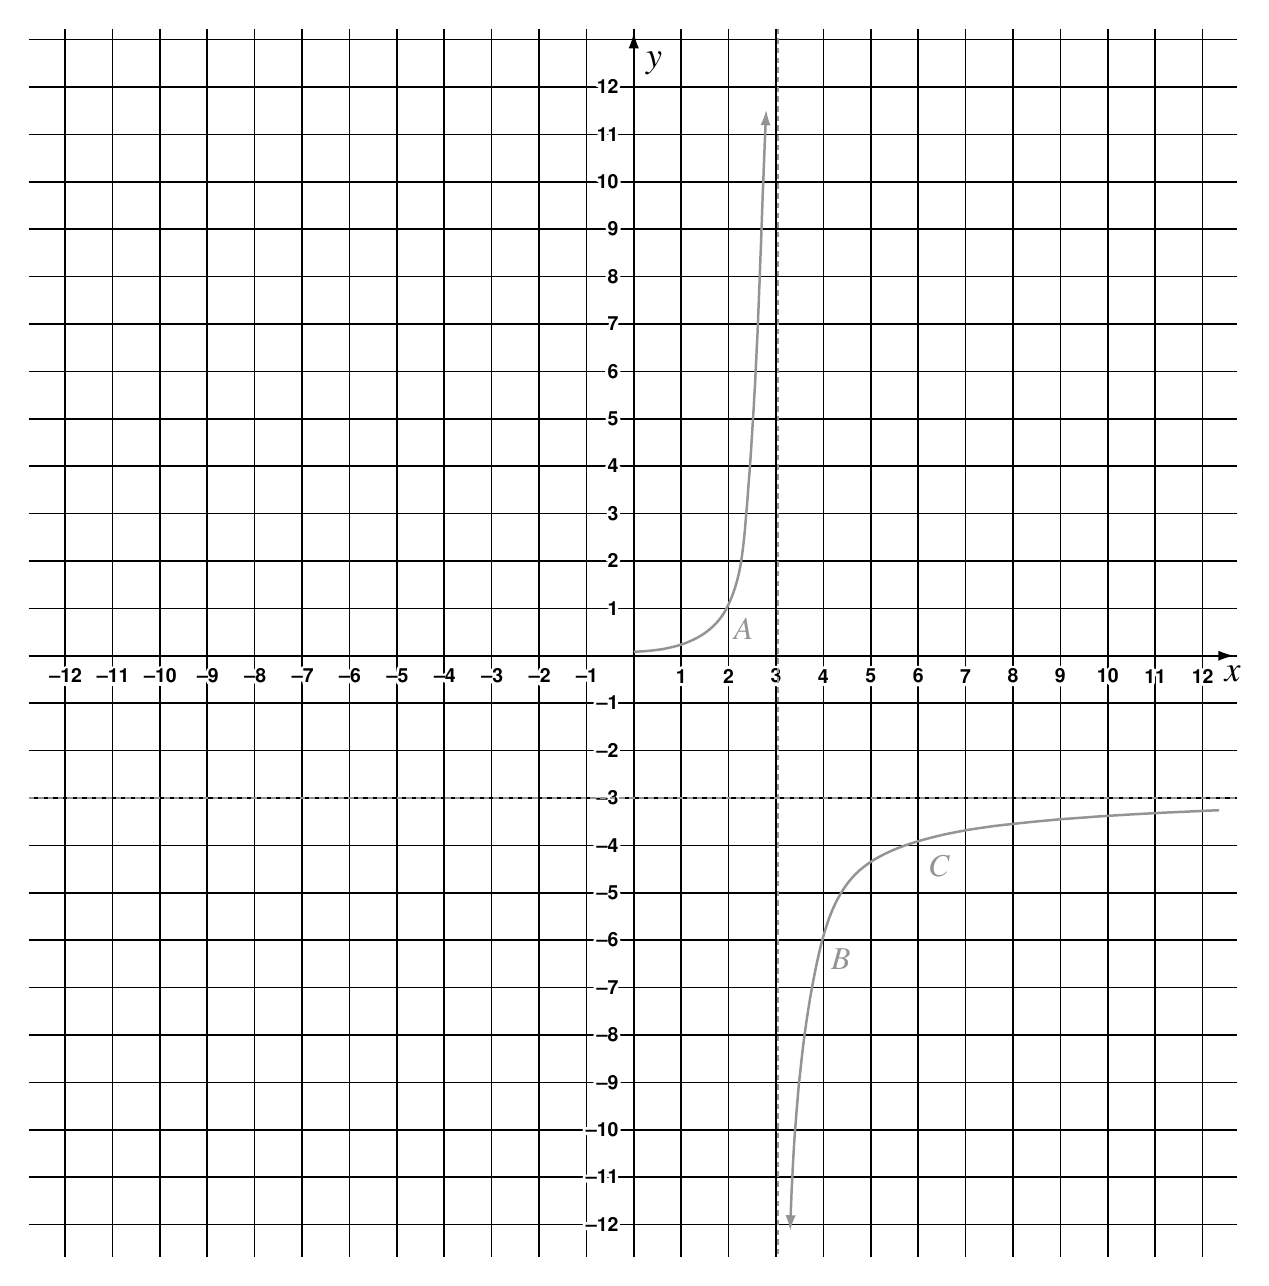
\begin{tikzpicture}[x=0.0127cm,y=-0.0127cm, every node/.style={inner sep=0pt},
  tl/.style={font=\sffamily\bfseries\fontsize{7.4}{8}\selectfont}]
  % grid
  \foreach \k in {-12,...,12} {\draw ({612.5+47.42*\k},5) -- ({612.5+47.42*\k},1234);}
  \foreach \k in {-12,...,13} {\draw (7,{632.5-47.42*\k}) -- (1216,{632.5-47.42*\k});}
  % axes
  \draw[->] (7,632.5) -- (1213,632.5);
  \draw[->] (612.5,1234) -- (612.5,9);
  % tick labels (grid stops around the digits)
  \foreach \k in {-12,...,-1} \node[tl] at ({612.5+47.42*\k},653) {\halo{$\boldsymbol{-}$\kern-0.5pt\number\numexpr-\k\relax}};
  \foreach \k in {1,...,12} \node[tl] at ({612.5+47.42*\k},653) {\halo{\k}};
  \foreach \k in {1,...,12} \node[tl, anchor=east] at (598,{632.5-47.42*\k}) {\halo{\k}};
  \foreach \k in {-12,...,-1} \node[tl, anchor=east] at (598,{632.5-47.42*\k}) {\halo{$\boldsymbol{-}$\kern-0.5pt\number\numexpr-\k\relax}};
  \node[font=\fontsize{13}{15}\selectfont, anchor=base west] at (624,44) {$y$};
  \node[font=\fontsize{13}{15}\selectfont, anchor=base west] at (1201,658) {$x$};
  % asymptotes (grey dashed, as printed)
  \begin{scope}[black!42]
    \draw[aux] (756.5,5) -- (756.5,1234);
    \draw[aux] (7,{632.5+3*47.42}) -- (1216,{632.5+3*47.42});
    \draw[->, line width=0.9pt] plot[smooth] coordinates {(612.5,628.5) (622.4,628) (631.8,627.1) (641,625.9) (649.7,624.1) (657.8,622) (665.6,619.3) (672.6,616.2) (679.3,612.6) (685.4,608.5) (690.8,604) (695.8,599) (700.1,593.6) (704,587.6) (707.5,580.7) (710.8,573) (713.7,564.7) (716.2,556.1) (718.3,547) (720,537.5) (721.4,527.5) (722.6,517.3) (723.7,506.4) (724.6,495.2) (725.6,483.9) (726.5,472.6) (727.3,461.3) (728.2,450) (729,438.8) (729.8,427.5) (730.5,416.1) (731.2,404.9) (731.9,393.5) (732.6,382.1) (733.2,370.9) (733.9,359.5) (734.4,348.2) (735,336.8) (735.5,325.5) (736.1,314.1) (736.6,302.7) (737,291.4) (737.5,279.9) (737.9,268.6) (738.4,257.2) (738.8,245.7) (739.2,234.4) (739.7,223) (740.1,211.5) (740.5,200.1) (740.9,188.6) (741.3,177.1) (741.7,165.8) (742.2,154.4) (742.6,143) (743.1,131.5) (743.5,120.2) (744,108.8) (744.5,97.41) (745,86)};
    \draw[->, line width=0.9pt] plot[smooth] coordinates {(1198,787) (1184,787.6) (1171,788.2) (1158,788.8) (1144,789.4) (1131,790.1) (1118,790.8) (1104,791.6) (1091,792.4) (1078,793.2) (1065,794.2) (1051,795.2) (1038,796.2) (1025,797.4) (1012,798.6) (998.6,800) (985.5,801.4) (972.6,802.9) (959.9,804.7) (947.4,806.6) (934.9,808.9) (922.7,811.4) (910.7,814.3) (898.8,817.5) (887.3,821.1) (876.3,825.1) (866,829.6) (856.3,834.6) (847.5,840.1) (839.5,846.2) (832.5,852.9) (826.2,860.4) (820.5,868.8) (815.3,878) (810.7,888) (806.7,898.5) (803.1,909.8) (799.9,921.5) (797,933.7) (794.3,946.3) (791.8,959) (789.5,971.6) (787.4,984.3) (785.4,997.3) (783.6,1010) (781.9,1023) (780.4,1036) (779,1049) (777.6,1062) (776.4,1076) (775.3,1089) (774.3,1102) (773.3,1115) (772.5,1128) (771.7,1142) (771.1,1155) (770.4,1168) (769.9,1181) (769.4,1195) (769,1208)};
    \node[font=\fontsize{11.5}{13}\selectfont, anchor=base west] at (711,616) {$A$};
    \node[font=\fontsize{11.5}{13}\selectfont, anchor=base west] at (808,946) {$B$};
    \node[font=\fontsize{11.5}{13}\selectfont, anchor=base west] at (907,853) {$C$};
  \end{scope}
\end{tikzpicture}
\end{document}
